\documentclass[UTF8]{csoarticle}


\newtheorem{theorem}{定理}
\newtheorem{lemma}{引理}
\renewcommand{\proofname}{证明}
% 如果为英文文章,可以使用下面的定义(去除行首的注释符号%)代替上述中文定义
% \newtheorem{theorem}{Theorem}
% \newtheorem{lemma}{Lemma}

\begin{document}

%----------------------------------------------------------
% 1. 文章标头信息
%----------------------------------------------------------

\titleCHN{基于局部特征的图像重建算法研究}
\titleENG{Image Reconstruction Based on Local Features}
\authorCHN{王继哲\affil{1},李学明\affil{2}}
\authorENG{WANG Ji-Zhe\affil{1}, LI Xue-Ming\affil{2}}
\affiliationCHN{
    \affil{1} 北京邮电大学信息与通信工程学院,北京 100876 \\
    \affil{2} 北京邮电大学信息与通信工程学院,北京 100876
}
\affiliationENG{
    \affil{1} School of Information and Communication Engineering, Beijing University of Posts and Telecommunications, Beijing 100876 \\
    \affil{2} School of Information and Communication Engineering, Beijing University of Posts and Telecommunications, Beijing 100876
}

\abstractCHN{基于局部特征的图像重建算法是利用原始图像的局部特征信息,以大规模图像集为数据源,进行较为精确的图像重建工作,使重建后的图像与原始图像相似,并且图像质量达到人眼主观效果较好的程度。本文首先对目前图像重建算法加以概述,综合介绍重建系统中的局部特征、视觉词组、部分相似图像搜索、特征匹配与配准、匹配特征块筛选、图像融合等多种技术,并针对重建系统在大规模语料集场景下的应用特点,对上述环节进行完善,在匹配图像块筛选中提出阈值自适应算法,为重建提供了更有力的依据,提升了重建效果;}

\abstractENG{Local features based image reconstruction is an algorithm which uses local features information of the original image,together with the large-scale image dataset,to perform accurate image reconstruction so that the reconstructed image is similar to the original image and achieves good visual quality.Firstly,we summarize the current architecture of the image reconstruction system,including the technologies of local descriptors,visual word group,partial duplicate image retrieval,feature matching and registration,patch filtering and image fusion.Then we propose adaptive threshold validation in the process of patch filtering to optimize current system at the scene of large-scale corpus.The results demonstrate that the proposed method provides stronger reconstruction evidence and thus improve the performance.}

\keywordCHN{信号与信息处理;图像重建;图像局部特征;尺度不变特征变换}%二级学科 081002 
\keywordENG{Signal and Information Processing,Image reconstruction,local feature,SIFT(scale-invaiant feature transform)}
\cateidCHN{TP37}

\authorIntroduction{王继哲(1989-),男,硕士研究生,主要研究方向:多媒体通信,图像处理。通信作者:李学明(1969-),男,教授,主要研究方向:多媒体通信,图像处理。}
%\fund{***基金(00000000),***基金(00000000)}

\maketitle


%----------------------------------------------------------
% 2. 正文内容
%----------------------------------------------------------

\section{引言}

随着数字时代的不断发展,智能终端日益普及,终端应用的功能也日趋多样化,有一类应用服务规模迅速扩大,这一类型的应用采用相似的客户端-服务器(Client-Service,简称CS)技术架构——智能终端使用传感器采集图像数据,并通过网络向服务器实时传输,由服务器来处理数据,将处理结果反馈给终端用户。而图像应用的爆发式增长给人们带来了一个全新的挑战:图像信息的传输占用了大量的带宽资源。目前的解决方案是在终端对原始图像进行下采样和压缩编码,它产生的图像信息的损失大大降低了用户体验,而且传统的压缩编码算法占用了一定的CPU资源,压缩比不是很高,压缩后的图像数据量依然较大。

另一方面,大数据时代的互联网拥有无比丰富的图像资源,图像数以亿计,样式种类五花八门,每天还不断有用户贡献着高质量高分辨率的图像。从信息的角度来说,人们拍摄的每一幅图像中所包含的部分或全部内容几乎都可以在互联网上其它图像中找到。

以上两点观察启示我们打破传统的基于像素的图像压缩方法,采用一种全新的基于大数据集的外部图像压缩方法。在2013年6月有学者\upcite{Cloud}提出一种全新的压缩方式——基于云的图像编码。其核心思想是在客户端提取并编码发送少量的图像特征数据,并不传输图像数据本身,而在服务器端解码后利用特征数据在服务器的大图像数据集上匹配相似的图像,再利用相似图像进行图像的重建。图\ref{fig:overview}展示了这一CS模式。
\begin{figure}
\centering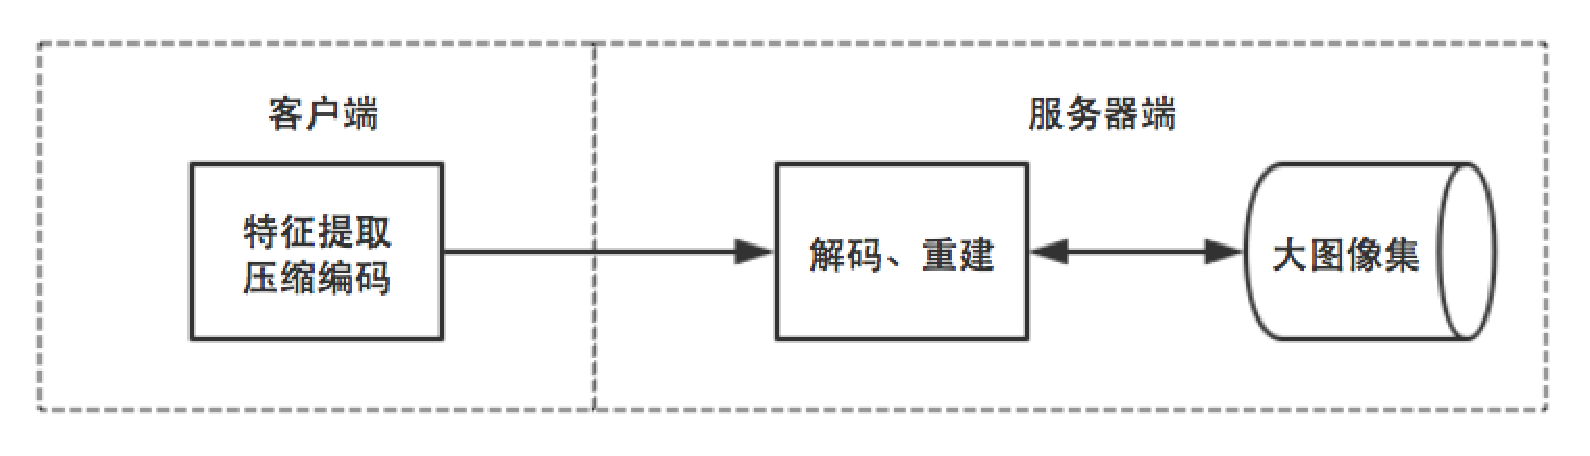
\includegraphics[width=12cm]{overview}
\caption{基于云的图像压缩模式}
\label{fig:overview}
\end{figure}
这种架构所运用的核心技术手段便是基于局部特征的图像重建算法,通过对原始图像进行特征提取与服务器端进行匹配与重建,用计算资源减少带宽损耗,从一个全新的维度进行数据压缩,为多媒体应用开启了一扇大门。本课题在这一成果基础上进行研究与完善,在相同的应用场景下着重探讨其中最为关键的图像重建环节。

\section{重建算法系统概述}
%介绍Cloud Coding 系统的概要
文献\cite{Cloud}创新性的提出了基于云的图像编码方式,以图像重建的方式取代了图像压缩编解码的传统流程,重建的大体流程如图\ref{fig:flow}所示。

\begin{figure}
\centering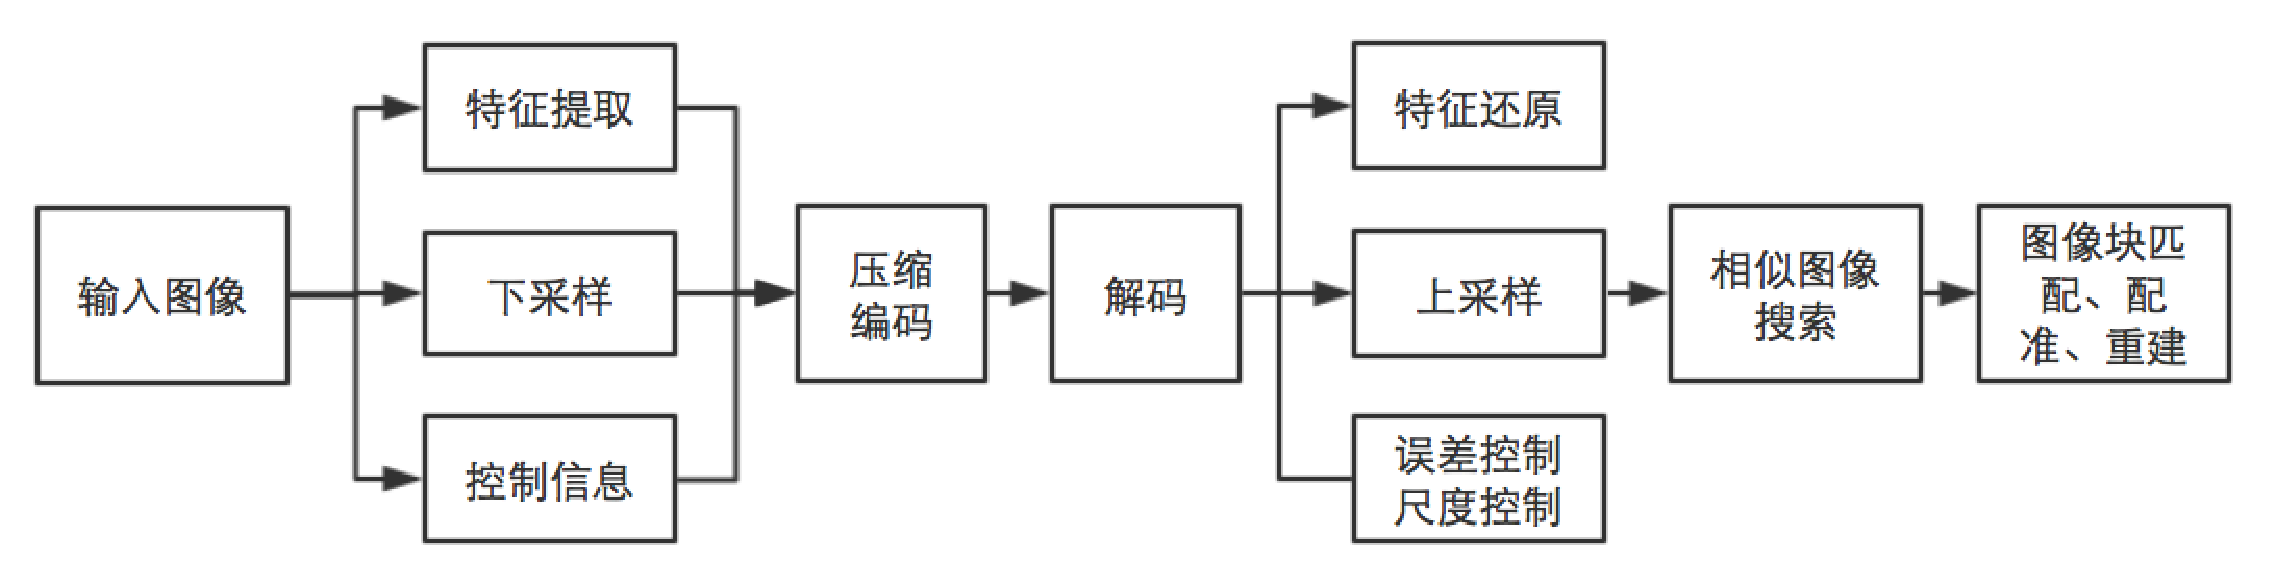
\includegraphics[width=15cm]{flowchart}
\caption{重建算法流程图}
\label{fig:flow}
\end{figure}

用户拍摄照片后,由客户端完成图像的局部特征提取,图像下采样,控制信息计算等一系列操作,经过复杂的变换、压缩编码后发送到服务器端。

服务器端对数据进行解码得到有损的特征数据、上采样图像以及控制信息,通过这三类数据在服务器端的大规模图像数据集上进行图像重建的工作。

\section{基于局部特征的图像重建算法}
在大语料集的应用场景下,图像重建的部分任务可以看成是多幅图像全景图拼接问题。与文献\cite{Brown:2006ir}中的流程类似,主要包含以下几个环节:(1)使用具有不变性的特征来描述图像;(2)自动找到图像之间的空间位置关系,进行图像配准;(3)图像融合,消除不同来源图像之间的光照差别,去除边缘噪声。

与全景图拼接不同的是,本文的图像重建系统首先需要在大规模图像数据集上进行相似图像搜索来确定拼接候选图像,进而依据上采样图像,以图像块(Patch)为单位进行图像匹配,配准及融合,如何解决图像块尺寸不一致、空间位置存在偏差等问题以及如何充分利用上采样图像信息优化图像融合是本文探讨的重点。现将系统中技术环节分别介绍如下:

\subsection{图像的局部特征}
局部特征是反映图像某一局部关键特性的一种描述,它是计算机视觉领域的基本问题。对局部特性进行描述需要解决的核心问题是如何反映出这一局部的不变性和可区分性。

在多种局部特征中,本文选择使用Lowe提出的尺度不变特征变换\upcite{sift}(Scale Invariant Feature Transform,以下简称SIFT)。SIFT算子具有很强的可区分性,同时对尺度、旋转以及一定视角和光照变化等都具有不变性。

\subsubsection{尺度空间理论}
尺度空间是对图像多尺度特征的一种模拟,尺度空间理论认为根据观察尺度的不同,自然界中的物体表现出不同的特性。比如我们观察一棵树,如果在几米在几百米的范围内观察它,会表现出树的特性; 在几微米的距离观察它,表现出分子的特性;在几公里外观察它,则表现出森林的特性。

在尺度空间中,图像模糊程度的逐渐增大能够模拟人在距离目标由近到远时目标在视网膜上的成像过程。已证明,高斯核是唯一的尺度空间核,因此一个图像的尺度空间\(L(x,y,\sigma)\)定义为原始图像\(I(x,y)\)与一个可变尺度的二维高斯函数\(G(x,y,\sigma)\)的卷积运算:

\begin{equation}
  L(x,y,\sigma) = G(x,y,\sigma) \otimes I(x,y)
\end{equation}

这里的高斯核参数\(\sigma\)反映出卷积运算对原始图像的模糊程度,也就是尺度空间的“尺度”。由于\(\sigma\)是连续的,所以尺度空间也是连续的。在尺度空间的任意两个尺度之间,有无数个平面,每个平面上都可以计算相应的局部特征,该特征反映出原始图像在这一尺度上的局部特性。在尺度空间上的若干个离散的尺度上抽取出相应的模糊图像,按顺序层叠放置在一起,则构成了经典的高斯尺度空间图像金字塔,将原始的二维图像转换成了三维的表示,提供了更丰富的图像信息。为了便于计算,将高斯尺度空间上相邻两幅图像相减,得到高斯差分尺度空间(Difference of Gaussian),下面提到的SIFT特征就是在该空间上进行检测和描述的。

\subsubsection{SIFT检测子与描述子}
SIFT算法有两个关键步骤,一是检测“感兴趣”的“关键点”,二是描述这个“关键点”。SIFT关键点是精心选择的一组在高斯差分尺度空间上的极值点。该关键点表示成\((x_f,y_f,s_f,\theta)\),包含三个信息,分别是(1)亚像素精度的\((x,y)\)位置信息;(2)尺度大小\(s_f\),反映关键点局部的大小,同时决定了特征的覆盖范围,对后文图像块的计算起到重要作用;(3)所在高斯尺度空间上的主方向\(\theta\),该主方向是由一个高斯窗口函数计算得来,反映关键点所在局部的方向信息。

SIFT描述子根据关键点所在高斯尺度空间上某一局部和方向上的梯度信息计算得来,以直方图的形式对梯度信息做统计,最终将特征描述成一个128维的向量\(S\)。

\subsection{特征匹配}
从重建算法逻辑顺序来讲,重建系统需要先对原始图像特征进行量化、计算视觉词组,再使用视觉词组在大图像集上进行相似搜索,找到最为相似的若干张图像组成拼接候选图像集,在候选集上做精细的重建工作,后文会对上述技术做进一步的分析。

通过相似图像搜索获得与原图近似的图像后,需要精确的找到原始图像与候选拼接图像相匹配的特征点,对于请求特征描述\(S_q\)和候选特征集合中任意特征\(S_p\)而言,其匹配策略为:

\begin{align}
  M(S_q,S_p) = 
\begin{cases} 
\text{true}, & \mbox{if } S_p = S_{min}\text{ and }\frac{\text{Dis}(S_q,S_{min})}{\text{Dis}(S_q,\tilde{S}_{min})} > \frac{1}{C} \\
\text{false}, & \mbox{otherwise}
\end{cases}
\end{align}
其中\(\text{Dis}(\cdot,\cdot)\)表示两个特征描述子之间的相似性度量(例如欧氏距离),距离越大,相似性越小。\(S_{min}\)和\(\tilde{S}_{min}\)分别表示的是与\(S_q\)距离最近和次近的特征。而C是一个阈值常数,通常取1.5。当原图特征点比较多时,为了提升匹配速度和匹配精度,可以适当提高该常数。

匹配搜索采用k-d树\upcite{lihang}技术进行最近邻搜索。对于n个实例的k维数据来说,建立kd-tree的时间复杂度为O(k*n*logn)。时间复杂度比暴力法要降低很多。

\subsection{图像配准}
原始图像的SIFT特征\(S\)与候选图像中的特征\(\tilde{S}\)是经过特征点匹配后找到的一对匹配特征点,通过它们可得到两幅图像上一组对应的图像块,原图图像块\(P_S\)和候选图像块\(P_{\tilde{S}}\)。每组图像块均由两个正方形区域构成,他们在位置,方向和尺度上存在差异,我们希望对候选图像块做进一步的投影变换,使之与原图像在空间位置上相一致,这一环节叫做图像配准,配准算法的核心是找到合适的投影矩阵\(H\)。

每个图像块所覆盖的区域内,除了决定图像块本身的SIFT特征点外,还包含其它特征点,根据图像块大小和特征点分布的不同,一个图像块内包含的特征点个数通常在几个到数百个之间,我们充分利用两幅图像块内部的特征点信息来完成投影矩阵的计算。

文献\cite{Dai:2012vn}中提到两种配准方式:第一种方法是利用图像块的全部特征点信息,使用随机抽样一致算法\upcite{ransac},通过多次迭代找到准确度最高的单应矩阵(Homography),在模型确定以及最大迭代次数允许的情况下,RANSAC总能找到最优解,称这个最优变换矩阵为\(H\);第二种方法是直接法,只根据一对匹配的SIFT算子直接写出两个图像块之间的变换矩阵,计算效率高但误差较大,得到的变换矩阵称为\(H_0\),下面简要介绍直接法。

一对匹配特征块是由一对匹配的SIFT特征点构成的,利用两个特征点\(\tilde{S}=(\tilde{x}_f,\tilde{y}_f,\tilde{s}_f,\tilde{\theta})\)和\(S=(x_f,y_f,s_f,\theta)\)的位置、尺度和方向,可以通过下列公式直接写出变换矩阵\(H_0\):

\begin{align}
  H_0 = 
  \begin{bmatrix}
  \frac{\tilde{s}_f}{s_f} R & T
  \end{bmatrix}
\end{align}
其中
\begin{align}
  R = 
  \begin{bmatrix}
    \cos{(\tilde{\theta}-\theta)} & -\sin{(\tilde{\theta}-\theta)} \\
    \sin{(\tilde{\theta}-\theta)} & \cos{(\tilde{\theta}-\theta)} 
  \end{bmatrix}
\end{align}

\begin{align}
  T = 
  \begin{bmatrix}
    \tilde{x}_f - x_f \\
    \tilde{y}_f - y_f
  \end{bmatrix}
\end{align}

计算得到的\(H_0\)和\(H\)都可以作为图像块的变换矩阵,系统同时计算两个矩阵,比较其准确程度,一般情况下使用准确度高的变换矩阵。准确程度的比较依据上采样图像和配准图像块的均方误差,而上采样图像本身的精度损失导致误差估计不精确,所以当匹配块内匹配特征点多时,更倾向于使用RANSAC算法计算得到的变换矩阵,反之倾向于使用直接计算法。

\subsection{图像块筛选与自适应阈值算法}
将变换矩阵直接作用在匹配图像块上,得到配准后的图像块。配准后的图像块有其自身的方向、尺度、位置,图像块之间可能存在交叠。在特征分布密集区域,图像块有大量的重叠,并不需要对每一个候选图像块进行拼接融合。利用相似图像搜索得到候选图像,在候选图像中利用特征匹配找到原图像块匹配的候选图像块,虽然在SIFT描述子级别上两个候选图像块是匹配的,但无法保证像素级别上的一致。其中有些图像块与原图在像素值上存在较大的出入,需要利用上采样图像计算配准后的图像块与原图像块的误差,根据设定好的阈值\(\epsilon\)移除误差较大的图像块。

文献\cite{Dai:2012vn}中使用上采样图像\(I_u\)来校验候选图像块是否正确。校验规则为

\begin{align}
\label{eq:errorControl}
  \text{Verify}(P_{\tilde{S}}) = 
\begin{cases} 
\text{true}, & \mbox{if MSE} (T(P_{\tilde{S}}),P_S \in I_u) < \epsilon \\
\text{false}, & \mbox{otherwise}
\end{cases}
\end{align}

其中\(\text{MSE}(\cdot,\cdot)\)表示的是两个图像块的均方误差(Mean Square Error)。\(T(P_{\tilde{S}}\)表示对候选图像块进行透视变换,\(P_{S}\)是\(P_{\tilde{S}}\)经过透视变换后在\(I_u\)上的相匹配区域。\(\epsilon\)表示一个阈值常数,当两个图像块的均方误差大于该值时,判定为错误匹配,否则认为是正确匹配。这里的难点是误差阈值\(\epsilon\)的确定,阈值设定过大,错误匹配块无法筛掉,阈值设定太小,筛选掉相对准确的匹配块,导致最后拼合有缺陷。一般情况下根据经验人为的指定一个相对合理的阈值。

为进一步提高匹配的准确性,文献\cite{Dai:2012vn}对上述配准后的图像块使用基于图的图像分割方案,对每一个分割连通域做均方误差校验,相当于对图像块做进一步的细分,能够有效去除图像块中与原图不一致的部分。在实际测试中发现,一方面图像分割占用大量的计算资源,这主要是由于我们的重建图像和候选图像分辨率高,而图像分割时间消耗与图像像素数量成正比;另一方面分割导致图像粒度过细,验证步骤的误差存在难以保证筛选结果的准确,因此本文没有采用图像分割的方案,而是提出了一种自适应阈值的图像块筛选法。

我们发现在公式\ref{eq:errorControl}中,因为\(I_u\)是由原始图像经过下采样、编解码、再上采样得到,上采样图像与原始图像在各个区块本身包含了误差,而且误差的大小与每一幅特定的图像以及图像的降采样和插值方式有关。如果设定一个固定的阈值,对于有些请求图像来说,可能会筛掉正确的块,对于另一些请求图像,可能会保留错误的匹配块。实验表明并没有一个标准的经验阈值可以适用于各种类型的图像。

针对上述出现的阈值设置难题,本文设计了一种在客户端根据原始图像本身的信息对验证误差阈值进行调整的自适应方法,能够根据请求图像的不同动态的调整验证阈值。

原始图像高频区域的图像块经过降采样再插值后得到的图像块与原始像素值有了较大的区别,平滑区域图像块经过降采样和插值处理后像素值的整体变化较小,有着较小的误差。又因为原始图像和候选图像在局部区域上往往是透视的变换,两者在像素值的梯度场的变化基本一致,所以原始图像与上采样图像的误差也反映了候选图像与上采样图像之间的误差。

有些原始图像整体较为平滑,与\(I_u\)误差不大,能够较好的反映原图的像素信息,这类使用较低的误差阈值能够得到较好的重建效果,与此相反,有些图像整体或者局部包含大量高频信息,图像\(I_u\)经过了平滑处理在像素信息上有了较大的损失,再使用小的阈值会导致误筛掉正确的匹配块。
自适应阈值方法在客户端计算每一个原始图像块上,计算每一个图像块在上采样图像块和原始图像块上的均方误差,在所有的均方误差数值中选取一个适当的值作为基准误差,再根据服务器端匹配的候选区块数量附加上一定的宽容度。

自适应阈值的图像块筛选法步骤是:
\begin{enumerate}
\item 提取图像\(I\)的SIFT算子,保留其中大于指定尺度的SIFT算子;
\item 对原始图像\(I\)进行降采样、编码、解码、上采样,得到\(I_u\);
\item 计算每一个SIFT算子对应的图像块\(P_S\);
\item 计算每一个图像块在\(I\)和\(I_u\)上的均方误差,以统计量X作为基准误差\(\epsilon_b\);
\item 在服务器端利用候选相似图像集合进行特征匹配,根据匹配块的数量M,计算宽容度\(\frac{\epsilon_C}{M}\);
\item 得到最终的验证误差阈值为:
\begin{align}
\epsilon = \epsilon_b + \frac{\epsilon_C}{M}
\end{align}
\end{enumerate}

其中\(\epsilon_C\)为一常数,\(\frac{\epsilon_C}{M}\)的意义是当匹配图像块数量较少时,容许的宽容度增大,尽量保证匹配的图像块能够作为重建图像的一部分,当候选图像块较多时,宽容度变小,重建条件变得苛刻。在步骤四计算基准误差时,可以采取不同的策略,例如以最大值作基准误差,如果最大值与第二大的值之间的差值过大,说明最大值可能是异常点,可以将其移除后依次查找,也可以使用均值、中值或者其它统计量或者引入更为复杂的策略。

阈值自适应算法的优势是计算效率高,不占用带宽,为图像块的筛选提供了更多的依据。

\subsection{大规模相似图像搜索}

在服务器端的大规模图像数据集上,利用聚类方法对随机抽样的SIFT特征进行量化,生成视觉词码表。利用视觉词码表将所有图像的SIFT特征归类到其对应的视觉词,并用简单的空间编码将一个视觉词所覆盖范围内的所有视觉词组合生成一个视觉词组,利用倒排索引技术进行快速的视觉词组查询和打分,最终得到得分最高最为相似的候选图像。这是本文所采用大规模相似图像搜索技术。

对于每一个图像块而言,中心位置有一个视觉词,该视觉词的尺度与其覆盖范围(影响范围)成正比,在该范围内,有若干视觉词,我们将范围内的所有视觉词看做一个视觉词组(Visual Words Group)。我们希望将词组内的每一个视觉词分配一个编码x,表征这个词在视觉词组的相对关系,这样我们可以采用如下的规则进行匹配:

\begin{align}
\label{eq:rate}
E_m(G_x,G_y) = E_v(G_x,G_y) - E_r(G_x,G_y)
\end{align}

其中\(E_v(G_x,G_y)\)是能够匹配上的视觉词,这里匹配上定义为两个视觉词相同,并且含有相同的编码x。其中\(E_r(G_x,G_y)\)是错误匹配的视觉词,错误匹配是指两个视觉词相同,但是含有不同的编码x。

图\ref{fig:visual}显示了两个视觉词组进行匹配的方式。左侧是请求图像的某个视觉词组,右侧是候选图像的视觉词组,两个视觉词组的中心视觉词相匹配,箭头方向是中心视觉词的主方向,正方形区域大小反映中心视觉词的尺度大小。尺度越大,正方形区域越大,越有可能包含更多的视觉词。虚线将正方形区域分割成若干个小区域,每个小区域有一个标号,利用标号对每一个视觉词组进行编码。

\begin{figure}
\centering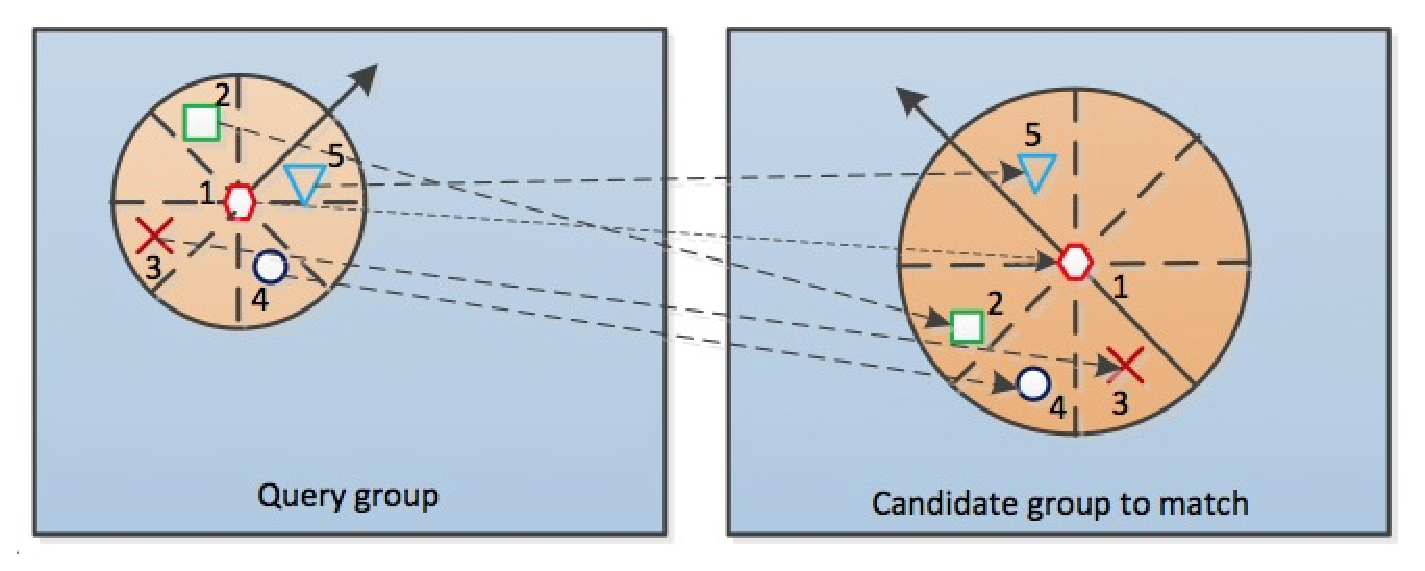
\includegraphics[width=12cm]{visual_group}
\caption{基于视觉词组的相似图像搜索}
\label{fig:visual}
\end{figure}

与经典的视觉词袋模型相比,使用视觉词编码的方式能够优先找到局部相似的图像,而不是全局相似图像。根据应用情景的不同,上述的二维编码可以划分多个图像区域,也可以加入区域内的其它特征点与中心特征点的相对尺度编码,进行更为精确的局部相似查询。

\subsection{图像融合}
在本文的图像重建系统中,图像融合是重建部分的最后一步,采用泊松图像编辑算法。泊松图像编辑是一种自动的“无缝融合”两张图像的技术,在文献\cite{Perez:2003ul}中首次提出。该方法所用的数学工具是带狄里克雷边界条件的泊松偏微分方程,狄里克雷边界条件指定了在影响域内未知函数的拉普拉斯算子,以及在区域边界上的未知函数值的拉普拉斯算子\cite{张建桥:2010vm}。

系统按照匹配块由大到小的顺序依次将其融合到上采样图像上,以上采样图像的像素值作为匹配块的边缘像素值,以匹配块的梯度场为指导,将边界上的差异平滑的扩散到融合后的图像块中。

\section{系统设计}

服务器端在线重建如图\ref{fig:serverOnline}所示。
\begin{figure}
\centering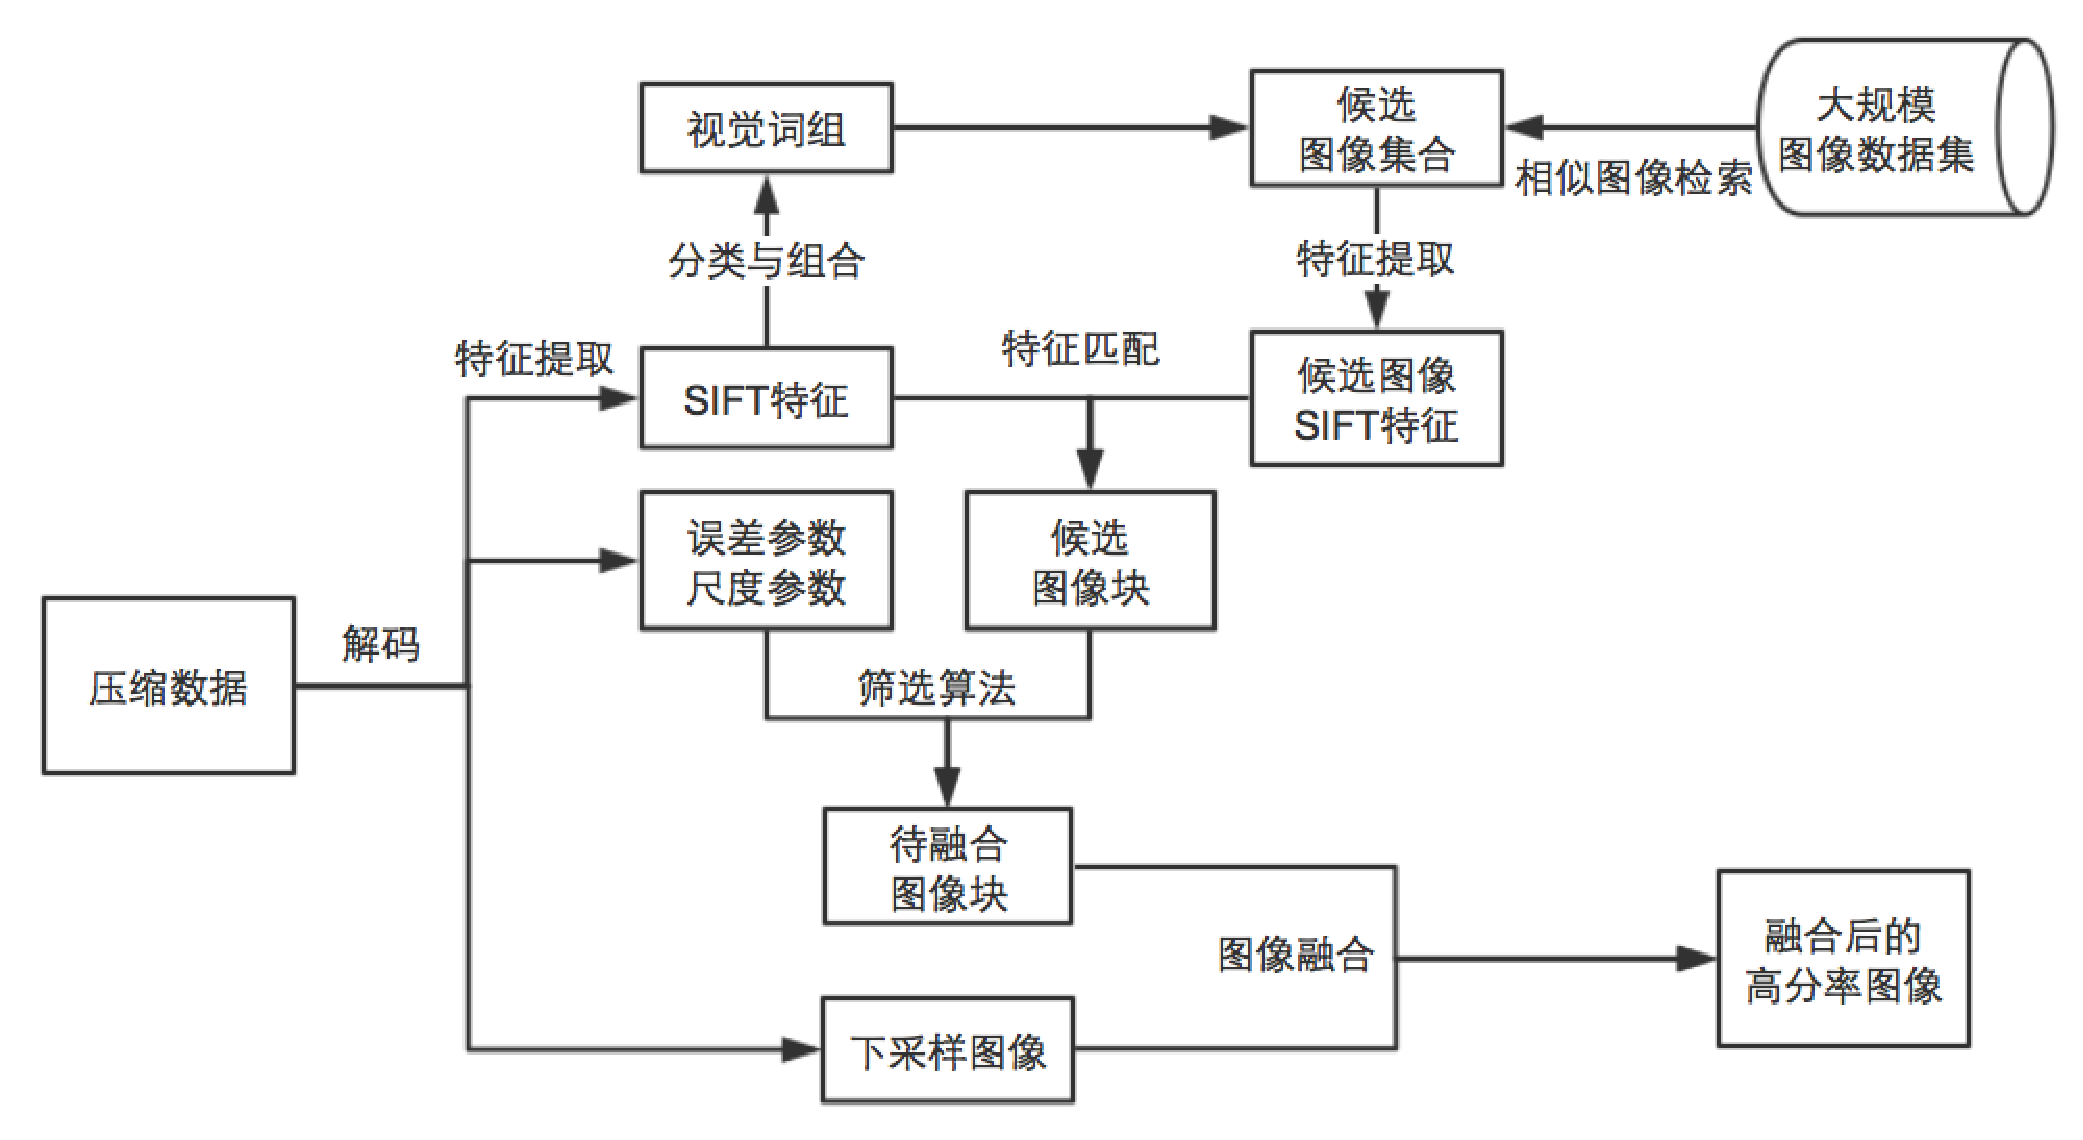
\includegraphics[width=15cm]{serverOnline}
\caption{服务器在线重建流程图}
\label{fig:serverOnline}
\end{figure}
从客户端传输来的压缩编码的数据包含了三部分信息,分别是(1)下采样图像,是1:256比例进行采样的图像,服务器端利用插值法进行上采样,恢复成原始大小得到\(I_u\);(2)SIFT关键点,传送给服务器的特征仅仅包含关键点的位置、尺度、方向等信息,不包含128维的描述子,服务器需要根据上述信息在图像\(I_u\)上重新计算特征描述,做进一步的匹配工作;(3)控制信息,包括误差控制参数中的基准误差和图像块的尺度控制等,尺度控制数值与客户端提取SIFT特征计算时有关,在客户端提取时一幅图像包含各个尺度上大量的SIFT算子,通常需要设定一定的尺度门限,只传输门限以上的特征,这个门限可以通过SIFT算子的数量不同动态的设定。

经过解码得到三类数据,运用上文提到的视觉词组编码方式计算视觉词组,在大规模图像集上利用倒排索引进行快速的相似图像搜索,得到了候选图像集合。对候选图像进行SIFT提取后与原始图像的SIFT进行匹配得到候选图像块,使用控制参数对候选图像块进行筛选得到待融合图像块,最后在下采样图像的指导下使用泊松图像编辑对图像块进行由大到小的融合,最终得到一幅高分辨率的重建图像。

\section{实验结果}
本文在Matlab和Python环境下仿真了上述的图像重建系统,使用VL-FEAT图像处理函数库
\cite{vl_feat}进行SIFT特征提取,使用其中相似K聚类(Approximately K-Means)进行视觉词的量化分类。本文使用INRIA Holiday数据集\cite{INRIA},该数据集包含了500组共1491张个人旅游照片,平均每幅图像的分辨率在五百万像素以上。选择其中三十张图像进行重建,其它图像作为大图像数据集进行训练。其中三幅图像的实验结果如图\ref{fig:result}所示。其中第一列是原始图像,第二列是采用较大数值作为误差阈值时的重建结果,第三列是采用较小数值作为误差阈值时的重建结果,第四列是采用自适应阈值法时的重建结果。

\begin{figure}
\centering
\includegraphics[width=15cm]{rec_result}
\caption{图像重建结果}
\label{fig:result}
\end{figure}

可以看到第一幅图像在阈值较大、误差条件宽松时对图像的重建效果好;第二幅像在阈值较小、误差条件苛刻时还原效果好;第三幅图像在误差阈值较大时出现错误匹配,而在较小时又有大面积的区域匹配不到任何候选图像块。采用自动阈值的方式进行图像重建,三幅图像的重建的效果均比较理想。实验结果表明,采用自动阈值进行候选图想块筛选的方式比固定阈值的图像块筛选方法要更加灵活,尽管不能保证每一幅图像都获得最佳的重建结果,但在大部分情况下能保证还原的图像有着较佳的主观视觉效果。

\section{结论}

本文对当前的基于云的图像重建算法中各个环节进行了深入的探讨,在其基础上针对大规模图像数据集应用场景进行了一定的完善。主要提出了自适应阈值的图像块筛选方法,实验结果表明:在不使用该方法时人工指定阈值在某些图像上能达到理想的还原效果,但在另外一些图像上则效果并不理想,结果数据显示由于不同图像之间不同区域的匹配块存在大量差异,没有一个固定的误差控制阈值能够适用于各类图像;而在重建系统中加入自适应阈值的方法,能够有效的找到合适的误差控制阈值,使得重建结果得到了提升,加强了图像重建系统的稳定性与适用性。

%----------------------------------------------------------
% 3. 参考文献
%----------------------------------------------------------
\begin{thebibliography}{10} % 这里的10是指参考文献总数目,需要根据实际情况进行修改
    \bibitem{Cloud} Huanjing Yue, Xiaoyan Sun, Jingyu Yang, and Feng Wu.Cloud-based Image Coding for Mobile Devices-Toward Thousands to One Compression, 2013.
    \bibitem{Brown:2006ir} Matthew Brown and David~G Lowe.Automatic Panoramic Image Stitching using Invariant Features.International Journal of Computer Vision, 74(1):59--73,December 2006.
    \bibitem{sift} Lowe D G. Distinctive image features from scale-invariant keypoints[J]. International journal of computer vision, 2004, 60(2): 91-110.
    \bibitem{lihang} 李航.统计学习方法[M],北京:清华大学出版社,2012.3
    \bibitem{Dai:2012vn} Lican Dai, Huanjing Yue, Xiaoyan Sun, and Feng Wu.IMShare: instantly sharing your mobile landmark images by search-based reconstruction.pages 579--588, 2012
    \bibitem{ransac} Fischler M A, Bolles R C. Random sample consensus: a paradigm for model fitting with applications to image analysis and automated cartography[J]. Communications of the ACM, 1981, 24(6): 381-395.
    \bibitem{Perez:2003ul} Patrick P{\'e}rez, Michel Gangnet, and Andrew Blake.Poisson image editing.ACM Transactions on Graphics (TOG), 22(3):313--318, 2003.
    \bibitem{张建桥:2010vm} 张建桥,王长元.基于泊松方程的数字图像无缝拼合,现代电子技术,2010,33
    \bibitem{vl_feat} Vedaldi A, Fulkerson B. VLFeat: An open and portable library of computer vision algorithms[C]//Proceedings of the international conference on Multimedia. ACM, 2010: 1469-1472.
    \bibitem{INRIA} H. Jégou and M. Douze, “INRIA Holiday Dataset,” 2008. [Online]. Available: http://lear.inrialpes.fr/people/jegou/data.php
\end{thebibliography}
\end{document}